\documentclass[]{template/llncs}
\usepackage{url}
\usepackage{graphicx}
\usepackage{amsmath}
\usepackage{amsfonts}
\usepackage[linesnumbered,ruled,vlined]{algorithm2e}
\usepackage[
colorlinks = true,
linkcolor = black,
anchorcolor = black,
citecolor = black,
filecolor = black,
urlcolor = black
]{hyperref}
\usepackage{xeCJK} 

\usepackage{fontspec}
\setmainfont{Times New Roman}

\begin{document}
\bibliographystyle{unsrt}
\pagestyle{plain}

%
\title{HashMix: Decentralized Cloud Hash Power Circulation Protocol (Draft)}

\author{HashMix Foundation}

\institute{
\email{dev@hashmix.org} \\
\vspace{0.5cm}
\today
}

\maketitle


\section{Background}

Ever since the release of the Bitcoin whitepaper by Satoshi Nakamoto, cryptocurrency projects using the Proof-of-Work (PoW) as a consensus mechanism have been mainstream in the industry. At the beginning of 2020, the circulating market value of Bitcoin and Ethereum using the PoW consensus mechanism has exceeded 700 billion U.S. dollars and 100 billion U.S. dollars respectively, jointly accounting for 80\% of the total market value of all blockchain projects with an annual output value of more than 15 billion U.S. dollars. Mining is the foundation of all PoW projects. By providing hash power, miners jointly maintain the security of Bitcoin and Ethereum, thereby earn block rewards and transaction handling fees. To some extent, the development history of the blockchain is the history of hash power competition. Hash power is the cornerstone of the security of cryptocurrency and important support for its huge market value. It can be predicted that in the future, the hash power market will inevitably continue to evolve as the blockchain develops and become one of the most important Internet infrastructures.

\subsection{Cloud hash power dilemma}

In recent years, as the blockchain industry prospers, miners have enjoyed tremendous industry dividends, and more and more people are attracted to PoW mining and want to be part of it. However, the research, development, production, and maintenance of mining equipment all require a high level of professionalism, making it difficult for most people to directly participate in the industry. Therefore, cloud hash power has become the easiest way to participate in mining for most people. For cloud mining products, the sellers are responsible for the operation and maintenance of the mining equipment, and the buyers pay the electricity bill and other costs generated during mining. Thus, buyers are relieved from the tedious work of maintaining the underlying mining hardware, meanwhile, receive the profits generated by the hash power they bought.

Traditional cloud hash power mostly adopts a centralized operation model, which means the hash power is owned by the retail platform or independent third party; besides, some miners are trying to issue centralized hash power equity tokens to provide cloud mining service in a new way. Although the two forms of cloud hash power are different, essentially they both require the credit endorsement of a centralized platform or a miner to ensure the delivery of hash power. However, due to the opacity of all operating details of the underlying mining hardware, the above-mentioned centralized cloud hash power platforms have the possible risks of oversold and fraud. When the cryptocurrency price fluctuates, it is likely for the buyers to have a hard time redeeming the hash power they bought, leading to systemic risks. Also, centralized cloud hash power products have no corresponding physical objects, thus the ownership cannot be confirmed, meaning there're potential legal risks.

Essentially, the mining machine itself is a device with powerful hashing capabilities. Therefore, people in the industry are also exploring more complex mining architectures to achieve efficient use of the bandwidth, storage, and hash capabilities of the mining machine. For example, Filecoin has achieved the innovation of Proof-of-Spacetime, thus for the first time, the on-chain measurement and proof of off-chain resource storage are realized, attracting many miners with high-end mining machines, who contribute multitudes of computation, storage, and bandwidth for the maintenance of the Filecoin network. To a great extent, this represents the direction of future blockchain development: more and more complex off-chain resources will be measured and coordinated on the chain through various advanced cryptographic technologies and become part of the Web3.0 infrastructure. This new type of mining model also brings new challenges to existing cloud hash power products: traditional cloud hash power products are too simple to cope with users’ demands across multiple dimensions such as “cloud sealing capabilities” and “cloud effective storage” on Filecoin, thus limiting the development of the emerging cloud hash power market.

\subsection{Liquidity bottleneck of hash power assets}

On the other hand, traditional mining machines and centralized cloud hash power, as assets, have almost no liquidity. Cloud hash power buyers can only hold hash power, can't change its ownership, therefore they cannot perform trading, lending, or any other financial operations with their hash power. This has greatly weakened the asset attributes of the hash power and restricted the further development of the hash power market. For mining machines and hash power holders, hash power assets with good liquidity can be easily sold or used as collateral; the risks on miners, sellers, and buyers of hash power can be lowered, and the utilization of funds can be improved through the combination of decentralized finance (DeFi) to provide hedging, quantitative trading, and other financial strategies. Besides, the current market design makes the pricing of hash power highly opaque. If the liquidity problem of hash power can be solved, more trading activities on hash power derivatives can be stimulated, so traders without physical hash power can also participate in the price discovery process, thus accelerating the commercialization of cloud hash power, which enables the entry of more funds into the hash power field. This is the prerequisite for the steady growth of global hash power in the future. Therefore, the industry is in urgent need of a set of decentralized solutions for hash power virtualization, trade, and lending, to enable the free circulation of hash power.

\subsection{Hash Power Isolation}

Most of the mining machines and hash power products are only for one single cryptocurrency, and there’s no easy way to change the mining target. The hash power of each cryptocurrency is isolated, which cannot form a greater interoperable network, which gives hash power owners very little flexibility. This is a key factor that prevents the hash power market from further growth: on the one hand, when the currency price experience extraordinary fluctuations, miners and cloud hash power holders will face the risk of hash power idling; on the other hand, idle hash power cannot switch to mine cryptocurrencies with a higher return. Thus, multi-target mining and the ability to switch mining targets become the basic needs of miners and cloud hash power buyers.


\section{Main contributions}

HashMix proposes a tokenization solution suitable for any hash power and implements a set of decentralized protocols with incentive mechanisms for general cloud hash power trading, lending, and swap to solve issues of hash power fraud, lack of liquidity and flexibility, allowing the free circulation of various forms of hash power beyond the geographical barriers. The main contributions of HashMix include the followings:


\subsubsection{Tokenization of hash power and corresponding on-chain proof}

HashMix utilizes multi-signature, smart contract, and cross-chain technology to generate and submit proofs of specific hash power product to the blockchain, tokenize hash power to NFT tokens to eliminate the necessity of centralized endorsement so that hash power can be circulated freely while the ownership of the hash power NFT holders is ensured; the proofs and smart contract can solve the hash power fulfillment problem;


\subsubsection{Decentralized cloud hash power trading protocol}

Based on the hash power NFT tokens, hash power can be traded in a decentralized manner. Traditional hash power for Bitcoin, Ethereum, and emerging Filecoin "cloud sealing capability" and "cloud storage power", all can be traded in a fully decentralized way without a trusted third party, while the security of hash power and trading funds is guaranteed.

\subsubsection{Cloud hash power lending protocol}

Based on the hash power NFT, hash power can be used as collateral assets to realize a lending market, reducing friction in the process of lending transactions and the pressure on the borrower's cash flow, and making optimal application of funds and resources.


\subsubsection{Ownership confirmation of cloud hash power}

Leveraging the characteristics of the non-fungible token (NFT), the cloud hash power is directly mapped to the physical mining hardware or storage resources in the real world, so it’s easy to confirm ownership, eliminating legal risks.

\subsubsection{Cloud hash power swap protocol}

Use hash power NFT to realize the swap of cloud hash power between different cryptocurrencies to increase flexibility.

\subsubsection{Incentive layer for cloud hash power circulation}

Design and implement an incentive mechanism and credit system for the tokenization, transaction, and circulation of universal cloud hash power, to motivate the various players in the ecosystem and ensure the operation of the protocol.

\section{System framework}

HashMix is a protocol for universal decentralized hash power tokenization that enables the circulation, trading, lending, and mining target changing. Its overall system framework is shown in the figure below:

\begin{figure}[htbp]
\centering
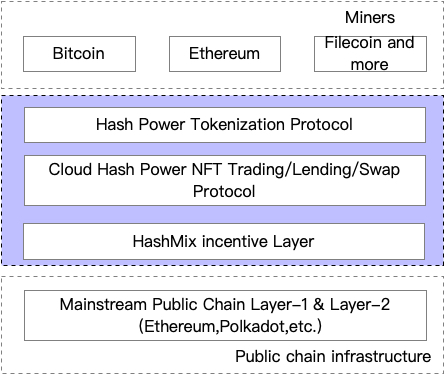
\includegraphics[width=0.9\columnwidth]{figure/system-architecture-en}
\caption{System architecture}
\label{fig:arch}
\end{figure}

At the top layer are various PoW mining projects, such as the traditional Bitcoin and Ethereum, and emerging mining architecture represented by Filecoin. These PoW miners will be connected through the HashMix protocol.

The middle layer is the core of HashMix protocol, consisting of the hash power tokenization protocol and the protocols for trading, lending, and switching, the former being the built-in foundation for the latter, and the HashMix incentive layer, which ensures the operation of the protocols. Among the protocols, the hash power tokenization protocol leverages multi-signature, smart contracts, and cross-chain technology to realize the NFT of hash power (such as hashing power of Bitcoin and Ethereum, and Filecoin’s capacity of sealing and effective storage power); cloud hash power trading protocol can enable the decentralized trading of the above-mentioned hash power NFT, and protect the rights and interests of both buyers and sellers; the lending protocol based on the cloud hash power NFT enables the borrowing and lending model based on hash power collaterals, and guarantees the security of the funds and hash power of both borrowers and lenders; the switch protocol based on the hash power NFT enables the free switches among different PoW projects. Through a set of economic incentive mechanisms (protocol fungible tokens), HashMix ensures that all stakeholders participating in the protocol jointly maintain the normal operation of the protocol.
 
The protocol interacts with the underlying public blockchain through smart contracts. With the help of the secure decentralized infrastructure of existing public chains (such as Ethereum and Polkadot), the issuance and circulation of hash power NFT are achieved, and a protocol incentive layer is realized while the hash power and transaction proof can be saved. The protocol can also be deployed on Layer 2, for example, using Rollup technology to realize off-chain hash power trading and save transaction records on a blockchain, thereby saving trading costs while ensuring decentralization and security. 

\section{HashMix ecosystem stakeholders}

Taking the typical hash power of Bitcoin and Filecoin mining as an example, the HashMix hash power ecosystem mainly includes the following stakeholders: 

\begin{figure}[htbp]
\centering
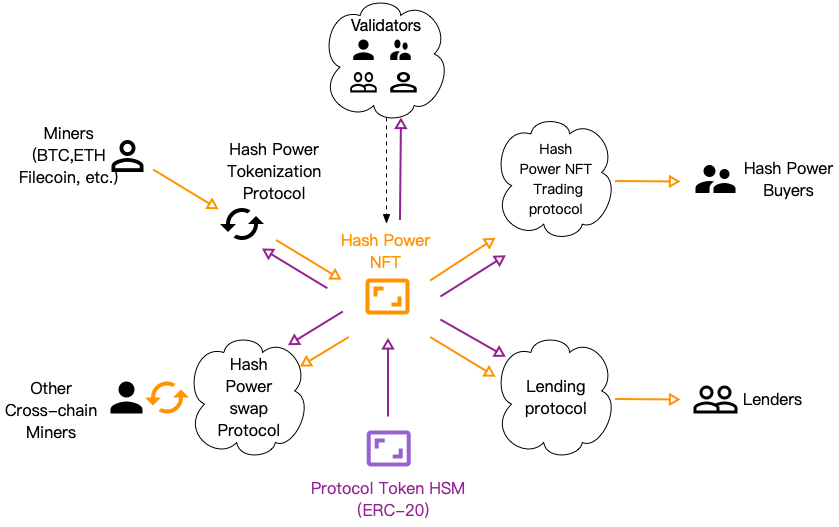
\includegraphics[width=0.9\columnwidth]{figure/HashMix-eco-new-en}
\caption{HashMix ecosysteme}
\label{fig:eco}
\end{figure}

\subsection{Miners}
Miners are the providers of hash power. They provide various types of hashing power in traditional PoW mining projects such as Bitcoin, and provide storage and computing resources in Filecoin, earning profits through mining. In the HashMix ecosystem, in addition to participating in the mining themselves, miners can also use hash power for staking, sell its hash power, collateralizing, or switching hash power to mining another cryptocurrency, etc.

\subsection{Cloud hash power buyers}

These buyers are users who purchase cloud hash power. Buyers of cloud hash power fall mainly into two categories. The first type purchases cloud hash power mainly for their use, so that they can participate in mining or staking using such cloud hash power to obtain benefits; the second type holds cloud hash power and sells it when the price rises, thereby earning the price difference.

\subsection{Lenders}

Miners or cloud hash power holders can use their cloud hash power as collateral to borrow funds from lenders to further expand their mining scale or make other investments. In return, the lenders receive loan interest accordingly.

\subsection{Validators}

At different stages of network development, the validators of the HashMix protocol can be reputable community leaders or participants of a fully decentralized community, responsible for validating the implementation of the various HashMix protocols, and arbitrating, when disputes are arising from the hash power transaction and loan process. Validators that meet the requirements can obtain corresponding protocol token rewards by participating in protocol verification.

Motives for participating in mining vary, but all the stakeholders use the hash power NFT as the link and are closely connected through hash power trading, lending, and switch protocols, thus jointly shaping a complete cloud hash power ecosystem.

The followings are brief introductions to the tokenization of hash power and the trading, lending, and switch protocols.

\section{Decentralized hash power tokenization protocol}

Before miners sell or deposit cloud hash power as collateral, they need to tokenize the hash power and turn the cloud hash power into hash power NFT that can be circulating. Most of the existing hash power tokenization schemes are based on collaterals, where the validity of the issued hash power tokens is guaranteed through centralized credit endorsements. Although this solution is simple to implement, there are hidden risks such as hash power fraud, unredeemable hash power, and unpromised gain since the real-world mining machines are not bound at all to the hash power tokens issued.

HashMix proposes a completely decentralized hash power tokenization solution, which combines non-fungible token (NFT) with multi-signature to link the hash power of real-world mining machines to hash power NFT one-to-one. The issuance, circulation, and redemption of hash power NFT can be verified by anyone without the participation of any centralized authority necessary, so there’s no way for anyone to false claim and oversold hash power. The holders of the hash power NFT can directly obtain the mining rewards generated by their cloud hash power, without the need for having rewards issued through miners or cloud hash power sellers. Take Bitcoin's hash power as an instance, the protocol can be implemented using Ethereum's smart contract. The basic implementation method is shown in the figure:

\begin{figure}[htbp]
\centering
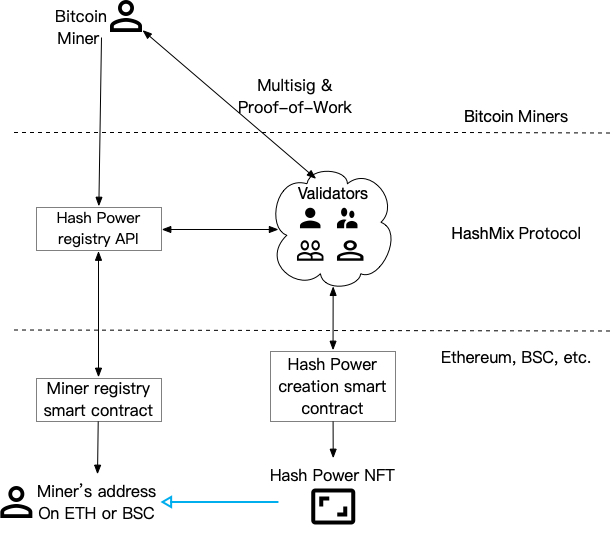
\includegraphics[width=0.9\columnwidth]{figure/Tokenize-new-en}
\caption{Tokenization}
\label{fig:tokenization}
\end{figure}

The miner owns hash power first registers in the smart contract deployed on Ethereum by HashMix, and binds his Bitcoin address to his Ethereum address. After that, the miner can send a request to HashMix protocol to tokenize their specific hash power. The validator of the HashMix protocol will call the corresponding contract on Ethereum to generate NFT for the Bitcoin hash power after the proof of work is verified, and send the NFT to the miner. Based on the information returned, the miner sets his reward receiving address for the corresponding hash power to a 2-of-3 multi-signature address (the addresses of the miners, NFT, and validators, among which the validator’s address itself is also a multi-signature address), and submits the proof for the corresponding workload. After the multi-signature address and the corresponding proof of work are verified, the hash power NFT will be sent to the miner's Ethereum address, and the hash power tokenization process completes.

The above hash power tokenization process is permissionless. Miners of any cryptocurrency (such as Ethereum or Filecoin miners) can generate corresponding hash power NFTs in a unified way. It is highly compatible with future mining formats that are getting increasingly complex (such as bandwidth, storage, and hash mining, etc.).

\subsubsection{Right to claim future earnings of NFT}

Through the aforementioned hash power tokenization protocol, HashMix sets the block reward address for the specific Bitcoin hash power to a multi-signature address (miner’s address, NFT holder’s address, and validator’s address). At this point, since the miner has both his address, which is a private key, and the newly generated hash power NFT, that means he is holding two valid private keys, so the miner has the complete right to claim the future earnings of the corresponding hash power, and any third party cannot hinder the miner from obtaining the block rewards generated from his hash power.

\subsection{Cloud hash power trading protocol based on hash power NFT}

After the hash power NFT is generated, miners can sell their hash power. Although the hash power NFT can also be directly traded like ordinary tokens, major disputes are highly likely to emerge in the transaction process. Since the hash power NFT only represents the right to the future income for the corresponding hash power, and the mining machines are still operated and maintained by the miners, so the cloud hash power buyers will bear the loss if the miners cannot cash in the hash power. The existence of validators in the multi-signature of HashMix can address this problem well.

\begin{figure}[htbp]
\centering
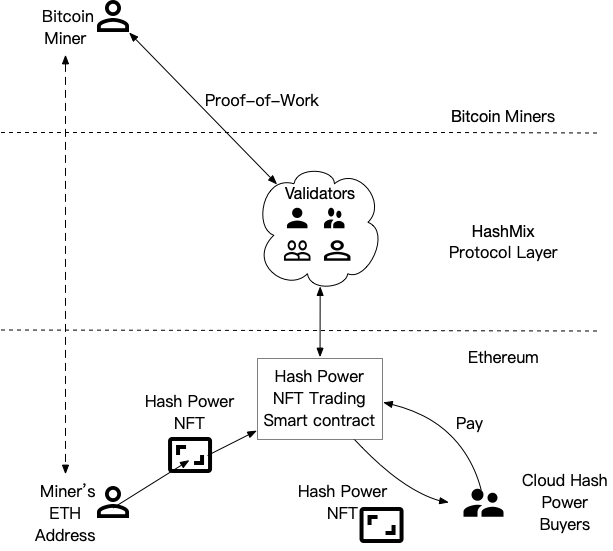
\includegraphics[width=0.9\columnwidth]{figure/nft-exchange-new-en}
\caption{HashMix NFT Exchange protocol}
\label{fig:exchange}
\end{figure}

HashMix has designed a standardized cloud hash power transaction protocol. When purchasing hash power NFT, cloud hash power buyers will not be paying the miners directly, but to a 2-of-3 multi-signature address (smart contract). The three-signature address is still composed of those of the miners, hash power NFTs and validators. Miners need to first send their hash power NFTs to the smart contract for cloud hash power trading, to initiate the transaction, then a multi-signature address will be automatically generated. After the buyer makes payments to the multi-signature address, the smart contract will send the hash power NFT to the buyer's address. The payment for the cloud hash power in the multi-signature address will be unlocked in installments at regular intervals throughout the cloud hash power service period agreed upon by the buyer and the seller. If there is no dispute between the buyer and the seller over the profits generated by the cloud hash power during the period, the two parties can use their multi-signature private keys to allocate the payments to the cloud hash power; if there is any dispute, the validators will verify the corresponding proof of work: If the workload meets the agreed hash power requirements, the unlocked funds will be sent to the miners with the joint decision by the miners and the validators; otherwise, the payment will be returned to the holder of the hash power NFT (i.e. the buyer). Through the HashMix NFT transaction protocol, the rights and interests of both buyers and sellers are protected, neither party could be able to obtain unjust benefits through cheating.

Holders of hash power NFT can also continue to resell cloud hash power. Since the multi-signature address does not involve the buyer's address but the address of the hash power NFT, no matter how the hash power NFT is circulated, the profits of the cloud hash power will only be sent to the current holder of the hash power NFT. Therefore, in the subsequent resale process, the hash power NFT can be freely circulated like an ordinary NFT, and its value mainly depends on the hash power and its remaining service period. Such information is recorded on the blockchain, and anyone can obtain information about any hash power NFT so that the market can complete the price discovery of hash power.

Through the HashMix hash power trading protocol, any hash power NFT can be freely circulated, and the right to obtain future income can be guaranteed without the need for a centralized third party.

\subsection{Lending protocol based on hash power NFT as a collateral}

Similar to hash power trading, lending protocol based on hash power NFTs as collateral can also be implemented through contracts. Miners borrow funds by pledging their hash power assets and use the upcoming cash flow generated by hash power to repay capital and interest. Taking Filecoin as an example, Filecoin miners can borrow a certain amount of FIL by pledging their hash power, in that case, they will have FIL token to meet the initial pledge collateral required for Filecoin mining. First, the Filecoin miner needs to convert his hash power into hash power NFT through the above-mentioned hash power tokenization protocol, and the owner address of the miner is a multi-signature address. Then, the miner or the holder of the hash power NFT can issue a borrow request through the HashMix lending protocol and send the corresponding hash power NFT to the HashMix lending contract. The lender sends the asset he wants to lend to the contract, then the contract will automatically send the hash power NFT to the lender, and send the borrowed asset to the owner address of the miner at the same time to complete the loan. Since the owner's address is jointly controlled by the miner, the hash power NFT (held by the lender), and the validator, so the loan is not at the disposal of any single party, thus the security of funds and collateral can be guaranteed without any over-collateralization.

If there is no dispute between the borrower and the lender, both parties can repay capital and interest through multi-signature according to the pre-agreed loan conditions; if there is a dispute, validators can come in for arbitration by verifying the proof of work of the hash power NFT and the dividends, then support for the transfer of funds in the multi-signature address to the performing party.

\subsection{Hash power NFT-based cloud hash power swap protocol}

HashMix supports easy to switch among different hash power, breaking the barriers among different hash power. No matter the miner is going to mine Bitcoin or Filecoin, the hash power tokenization process can be achieved in a standardized way in the HashMix protocol. Therefore, the NFTs that represent Bitcoin or Filecoin hash power is essentially the same, so they can be switched from one to another. There are mainly two ways to switch hash power:

\begin{itemize}
	\item Direct atomic swap. Bitcoin hash power NFT and Filecoin hash power NFT can be switched atomically through HashMix's hash power switch protocol. Both parties obtain each other's hash power NFT by the atomic swap transaction, thereby obtaining the subsequent benefits of the corresponding hash power NFT;
	\item Deposit into the hash power pool for the transaction. Holders of hash power NFT can deposit their hash power NFT into HashMix's hash power pool to obtain HashMix's native token HSM; then exchange HSM for other types of hash power in the pool. The pool adopts an automatic market maker model to provide liquidity for different types of hash power tokens.
\end{itemize}

\section{Incentive layer for decentralized hash power protocol}

The aforementioned hash power tokenization protocol and affiliated cloud hash power trading, lending, and switch protocols can enable the basic free circulation of hash power, thus solving many current pain points in the cloud hash power market. However, the hash power protocol brings in additional protocol consensus and requires a set of economic incentive mechanisms to encourage all stakeholders in the ecosystem to perform their duties by the protocol and jointly maintain the operation of the protocol. 

HSM is the native token of HashMix protocol which is used to incentivize all ecosystem stakeholders. The max supply amount of HSM is 1 billion. Among the total supply, 60\% of HSM will be generated through community mining and used to reward miners who maintain the operation by providing hash power, HSM and hash power NFT holders, hash power token and HSM liquidity providers, and validators who participate in the consensus process of the protocol. The other 40\% of HSM will be assigned to other contributors to the ecosystem. For specific token distribution and release rules, please refer to "HashMix Token Economy Whitepaper".

\begin{itemize}
	\item 40\% for community mining, including miners' hash power rewards, hash power NFT and HSM staking, hash power and HSM liquidity mining, and validators rewards, etc.;
	\item 15\% for the development team, lock for the first year, and vesting over 3 years from the 2nd year, for long-term project development;
	\item 3.3\% for Seed round Investors. Lockup for 6 months or upon listing on mainstream exchanges, then unlock 10\%, the remaining 90\% will be vesting for 12 months.
	\item 8\% for Private round Investors. Lockup for 6 months or upon listing on mainstream exchanges,, then unlock 10\%, the remaining 90\% will be vesting for 12 months.
	\item 6\% for Community and Ecosystem Developers. Will be used for long-term community incentives for active community members and developers.
	\item 27.7\% reserved for HashMix Foundation. This part is used for initial liquidity and miner incentives, exchange, legal, financial, and research cooperators, vesting for 4 years, determined by the whole HashMix ecosystem.
\end{itemize}

40\% of the total amount in the system needs to be generated through mining. There are four main ways of mining:

\begin{itemize}
	\item First, miners who have the hash power of various mainstream cryptocurrencies can pledge a certain amount of HSM to convert their existing hash power into the corresponding hash power NFTs. Miners who issue the NFTs through the HashMix protocol need to submit proof of their corresponding hash power continuously to obtain HSM rewards. If such proof cannot be provided, the upcoming reward will not be able to be obtained, and the pledged and locked HSM may be slashed.
	\item Second, for buyers who hold hash power NFT, in addition to obtaining the mining profits generated by their hash power, they can also stake their hash power NFT with their HSM to obtain HSM.
	\item Third, holders of hash power NFT and holders of HSM can provide liquidity for hash power NFT and HSM respectively, thereby obtaining HSM rewards.
	\item Fourth, by staking HSM, HSM holders can become HashMix's validators to verify hash power trading, lending, switching automatically in the network, and earn HSM fees and rewards. If the validator cheats, part of the staked HSMs will be slashed, and the remaining HSMs will be rewarded to Validators who have completed the validation correctly.

\end{itemize}

Besides, HSM holders can also participate in HashMix governance to jointly determine the direction of protocol upgrades and iterations.

27.7\% of the tokens will be reserved by the HashMix Foundation as long-term incentive, and the detailed usage will be determined by the whole HashMix ecosystem. 
The remaining 32.3\% of the tokens will be allocated to other contributors to the HashMix ecosystem, including team, investors, community KOLs and developers, etc. Together with the other incentives introduced above, they form the incentive layer of the HashMix protocol. For more details, please refer to the "Token Economy Paper".

\section{Roadmap}

\begin{itemize}
	\item Quarter 1, 2021
	\subitem Release “HashMix Technology Whitepaper” and “Token Economy Whitepaper” 
	\subitem Release HashMix project roadmap 

	\item Quarter 2, 2021
	\subitem Release FIL lending protocol based on Filecoin hash power 
  	\subitem Release prototype of the hash power tokenization protocol 
  	\subitem Enable HSM liquidity mining
 	\subitem HashMix official DAPP
 	
	\item Quarter 3, 2021
  	\subitem Launch Bitcoin and Filecoin hash power tokenization and trading protocol 
	\subitem Enable validator rewards and hash power mining 
  	\subitem Launch hash power wallet and other supporting utilities 
	\item Quarter 4, 2021
  	\subitem Launch decentralized hash power NFT lending protocol (Filecoin, Bitcoin, and Ethereum hash power)
	\subitem Enable universal NFT Staking
	\item Quarter 1, 2022
	\subitem Launch decentralized hash power NFT switch protocol
	\subitem Enable NFT liquidity mining
	\subitem Layer2 hash power NFT transaction, lending and exchange, etc.
	\item Quarter 3 and 4, 2022
	\subitem Hash power NFT-based derivatives, hash power pool-based standard hash power, hash power stable coin, etc. 

\end{itemize}

\section{Summary}

HashMix proposes a tokenization scheme suitable for any hash power and implements a set of universal decentralized cloud hash power trading, lending, and switch protocols through reasonable economic incentive mechanisms, to solve the issues in the current cloud hash power market like hash power fraud, lack of functionality, liquidity, and flexibility, thus allowing the hash power to circulate freely around the world.

\end{document}